\newlength{\twosubht}
\newsavebox{\twosubbox}

\begin{figure}

% preliminary
\sbox\twosubbox{%
  \resizebox{\dimexpr0.9\textwidth}{!}{%
    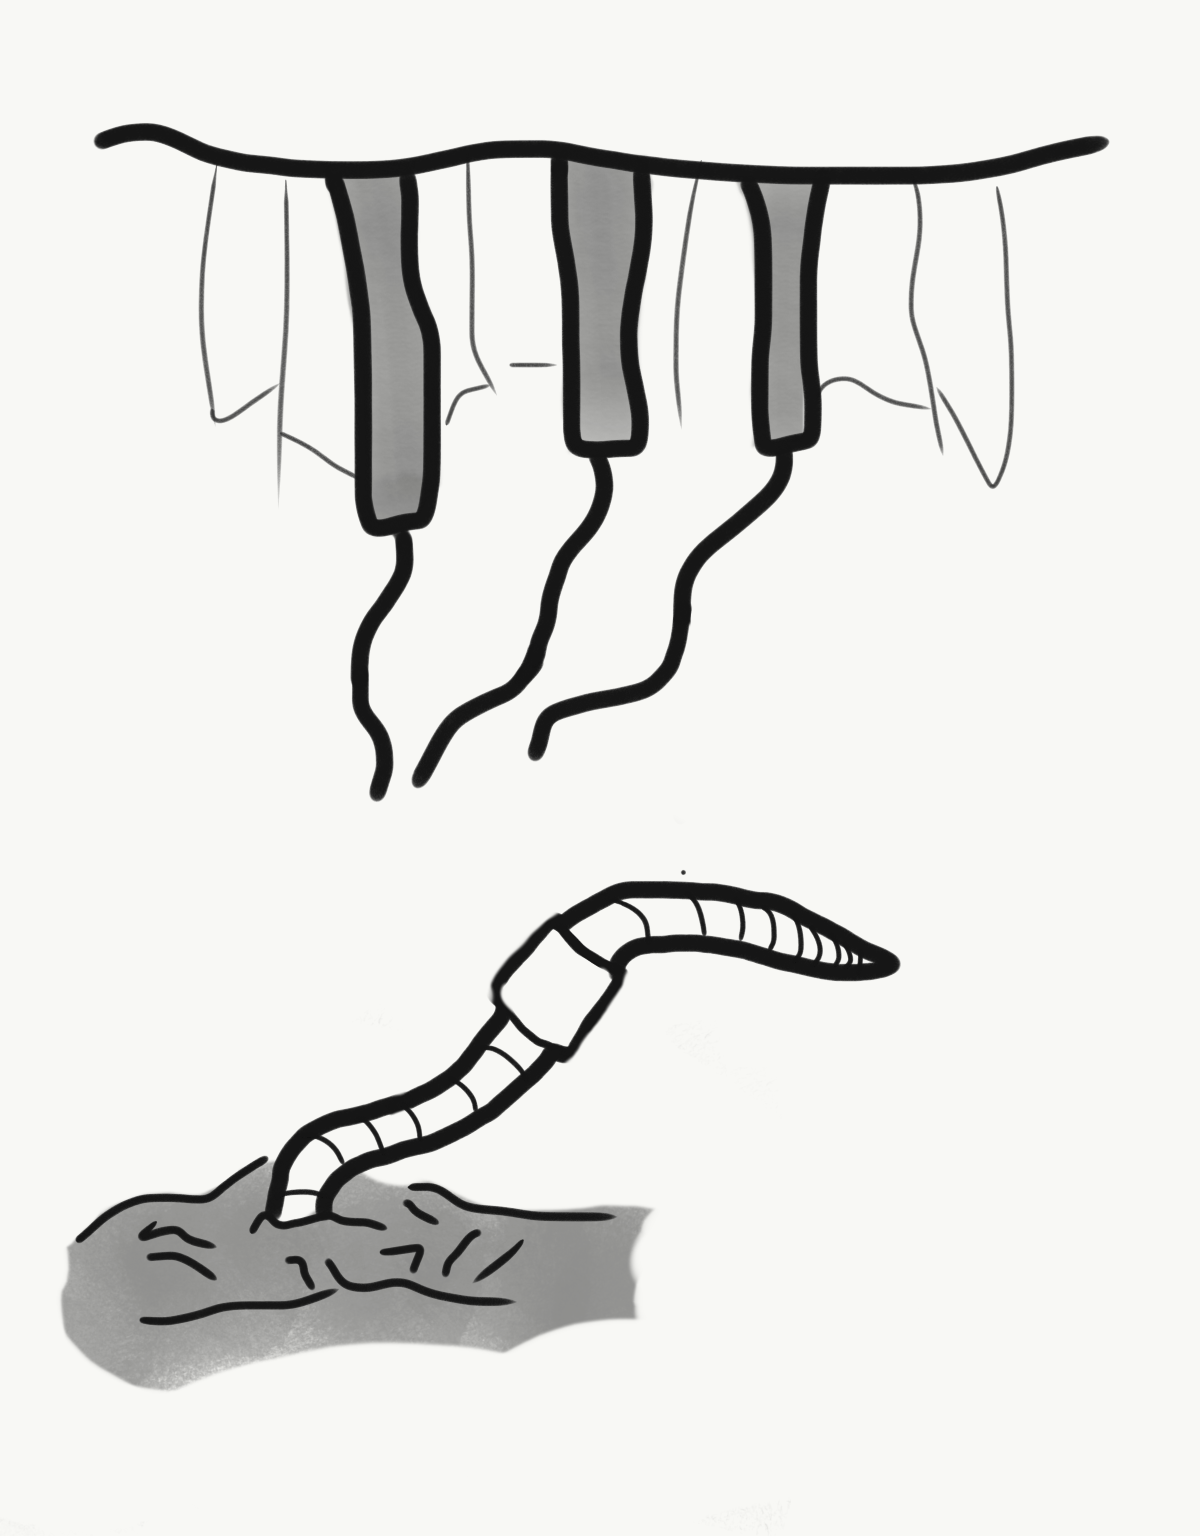
\includegraphics[height=3cm]{img/worm_eye}%
    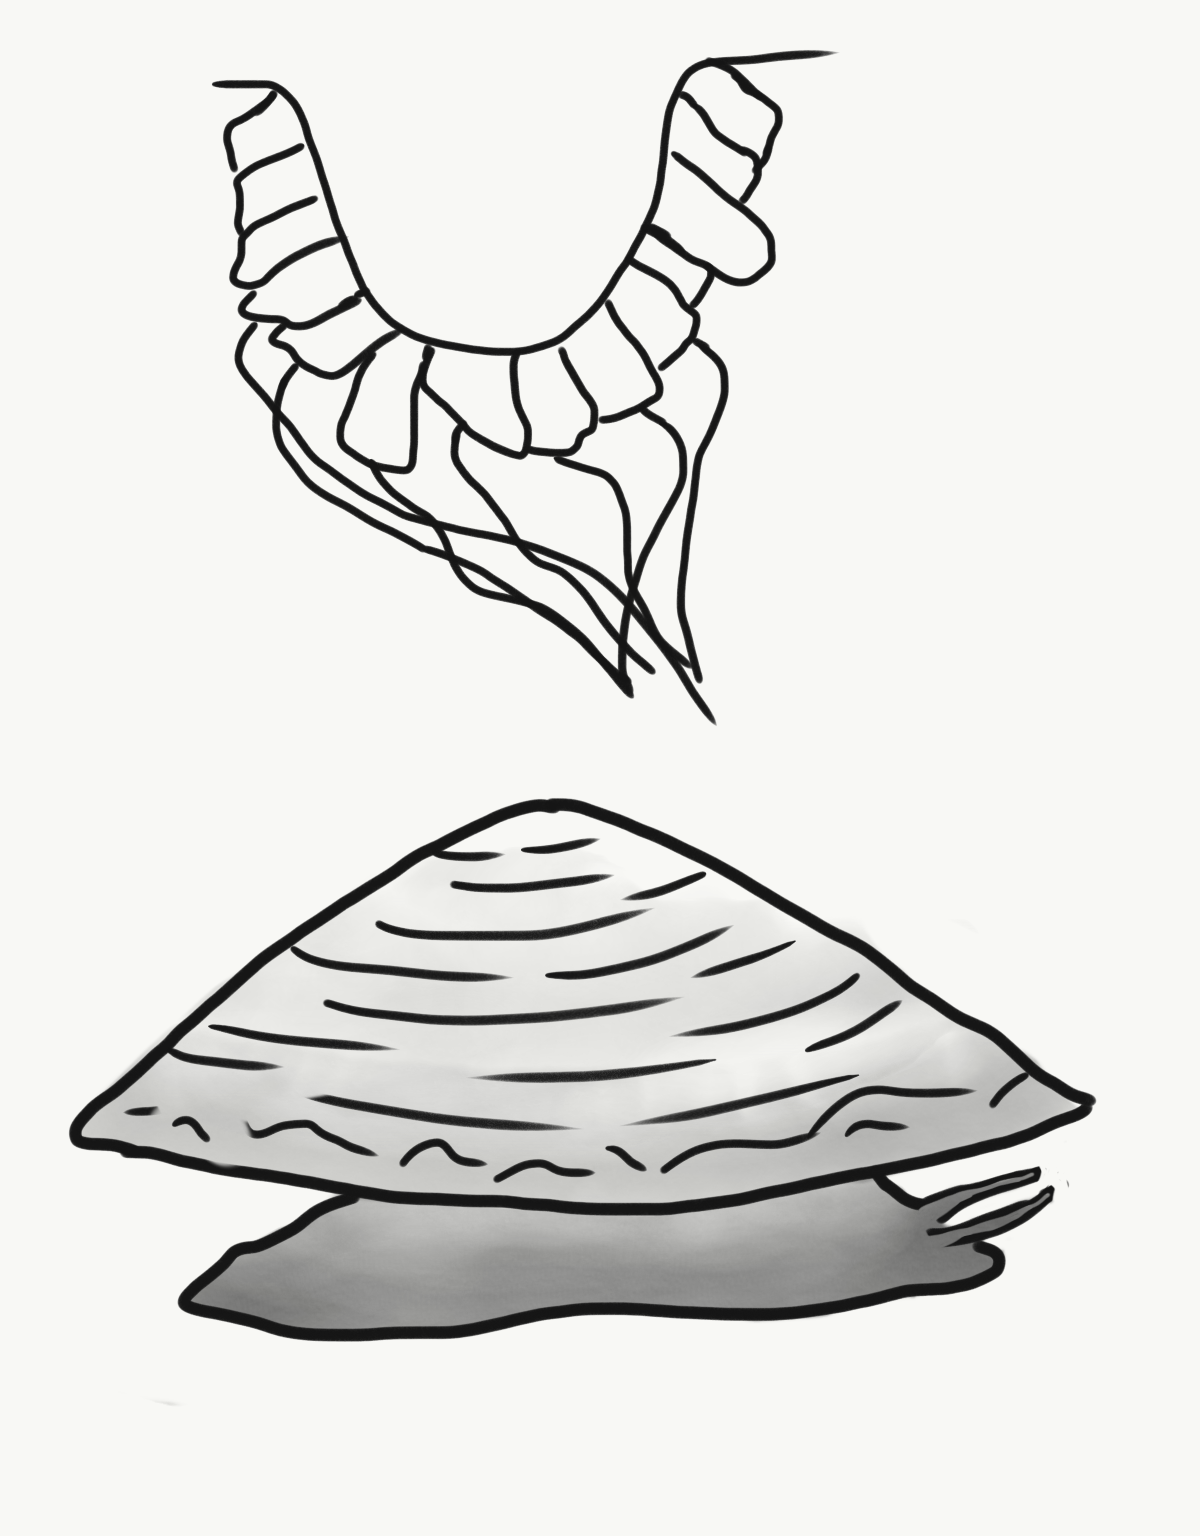
\includegraphics[height=3cm]{img/limpet_eye}%
    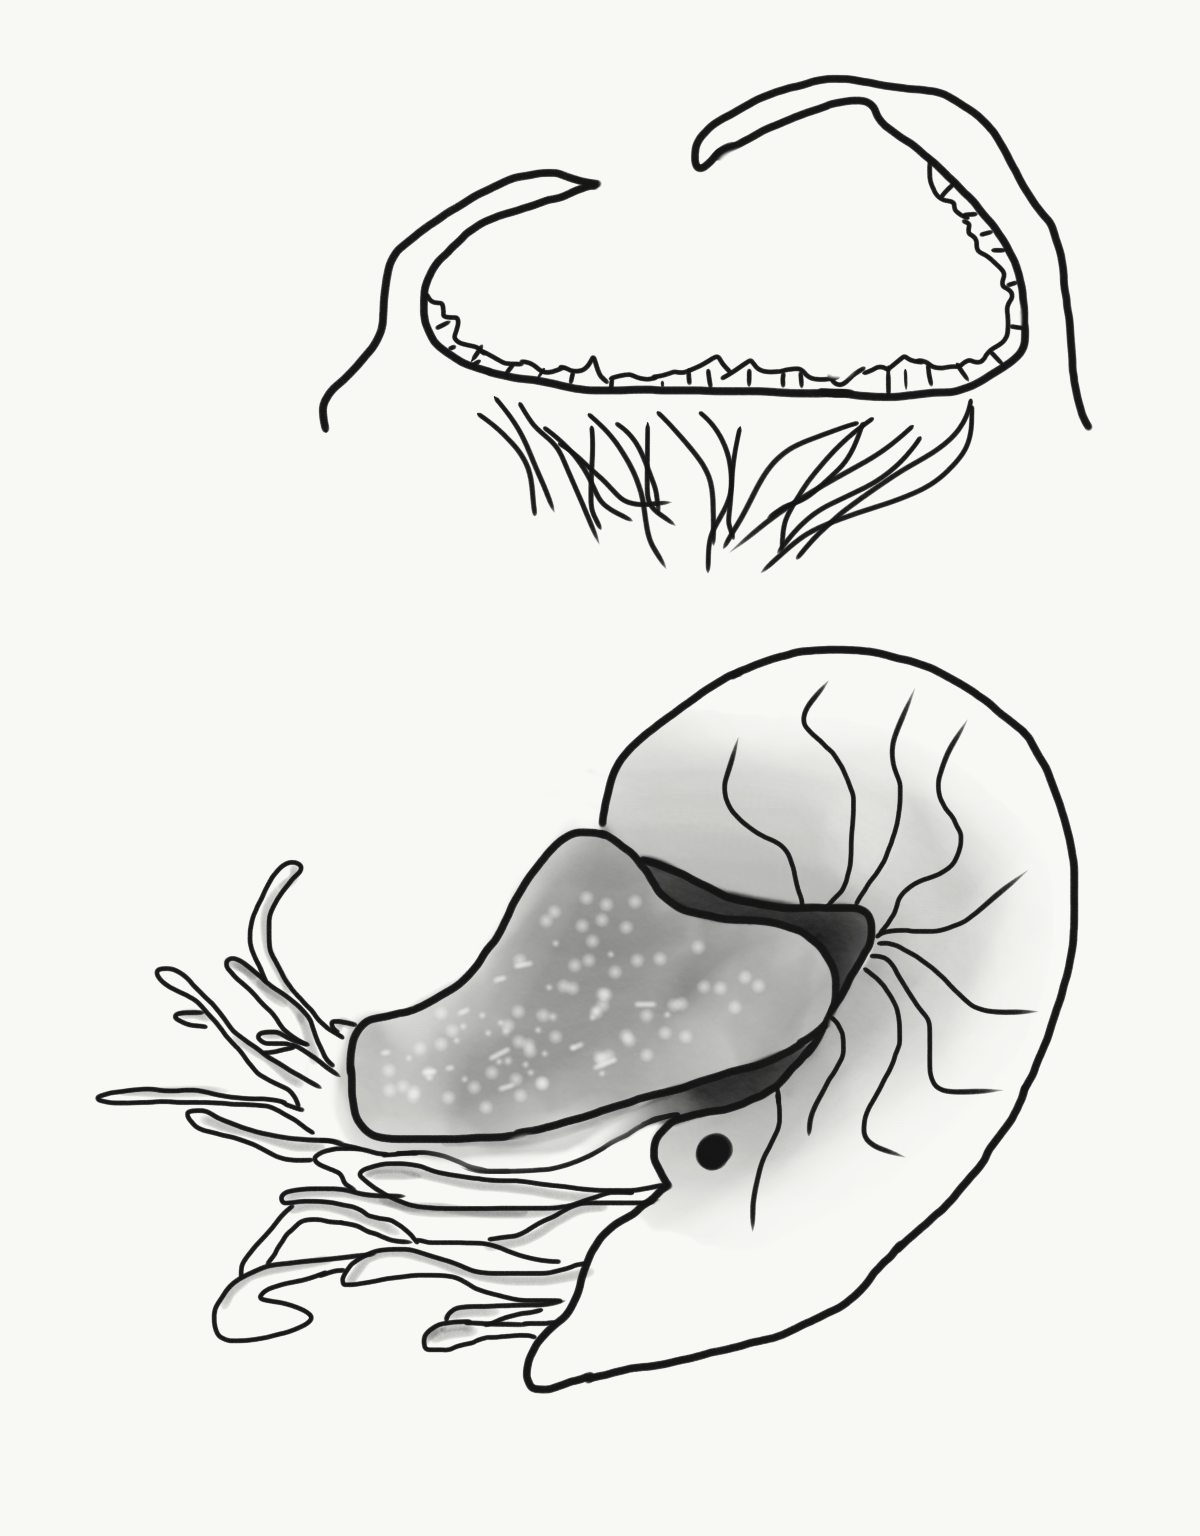
\includegraphics[height=3cm]{img/nautilus_eye}%
    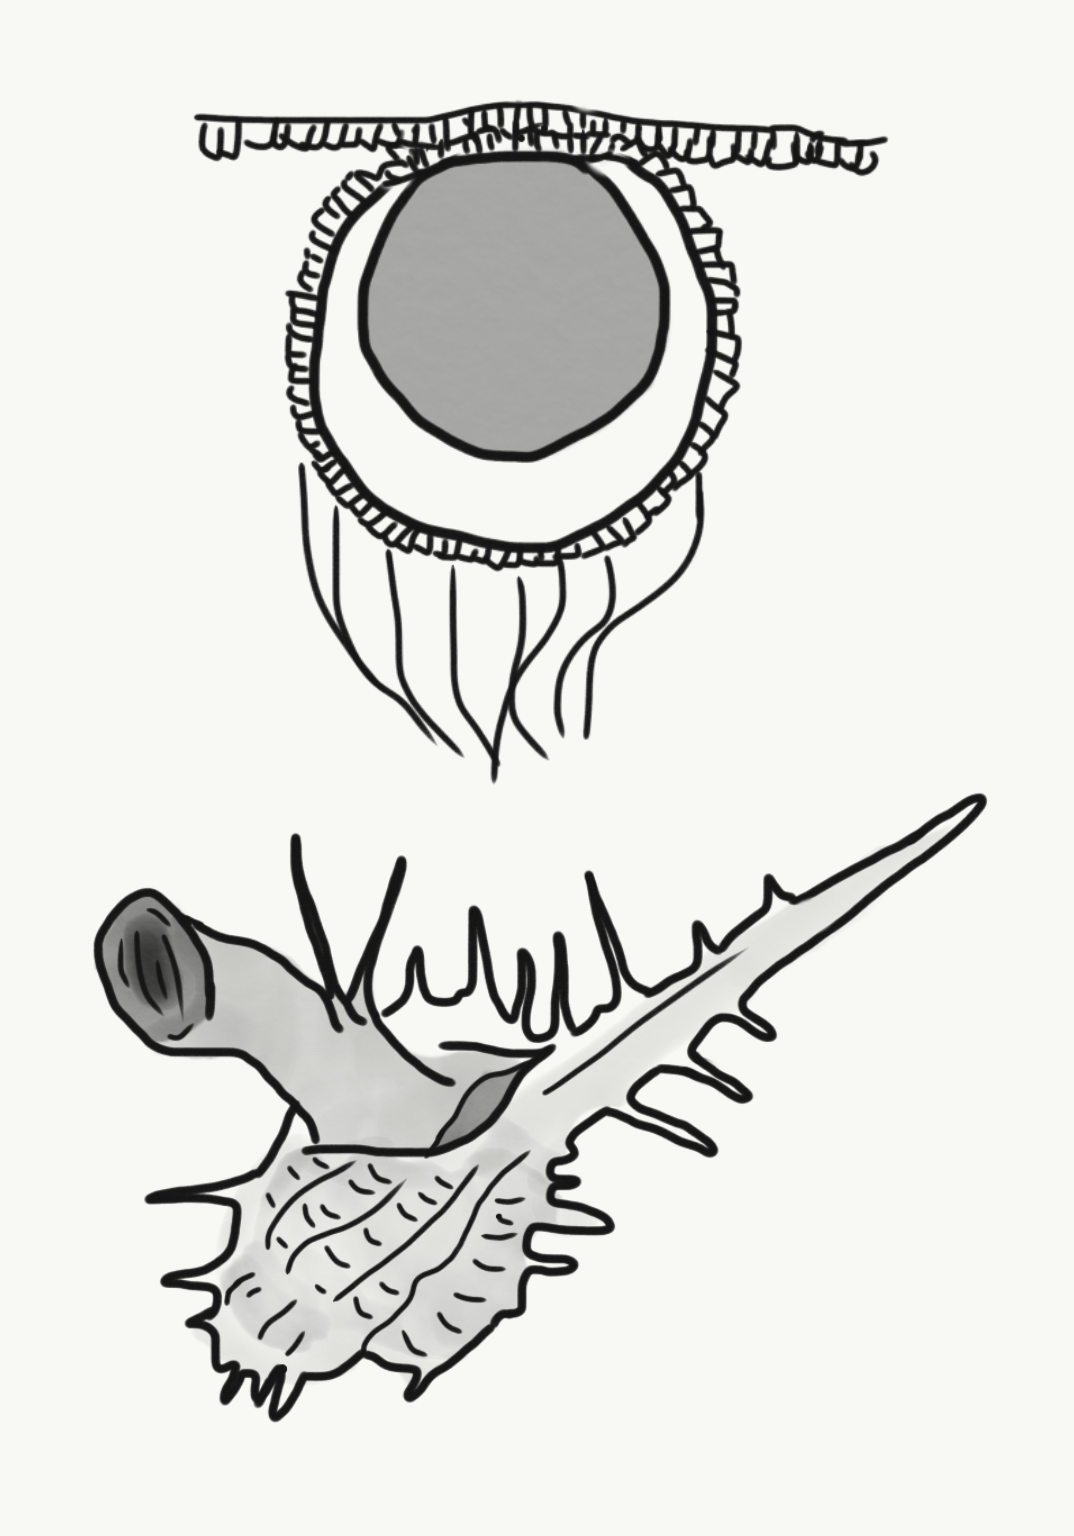
\includegraphics[height=3cm]{img/murex_eye}%
    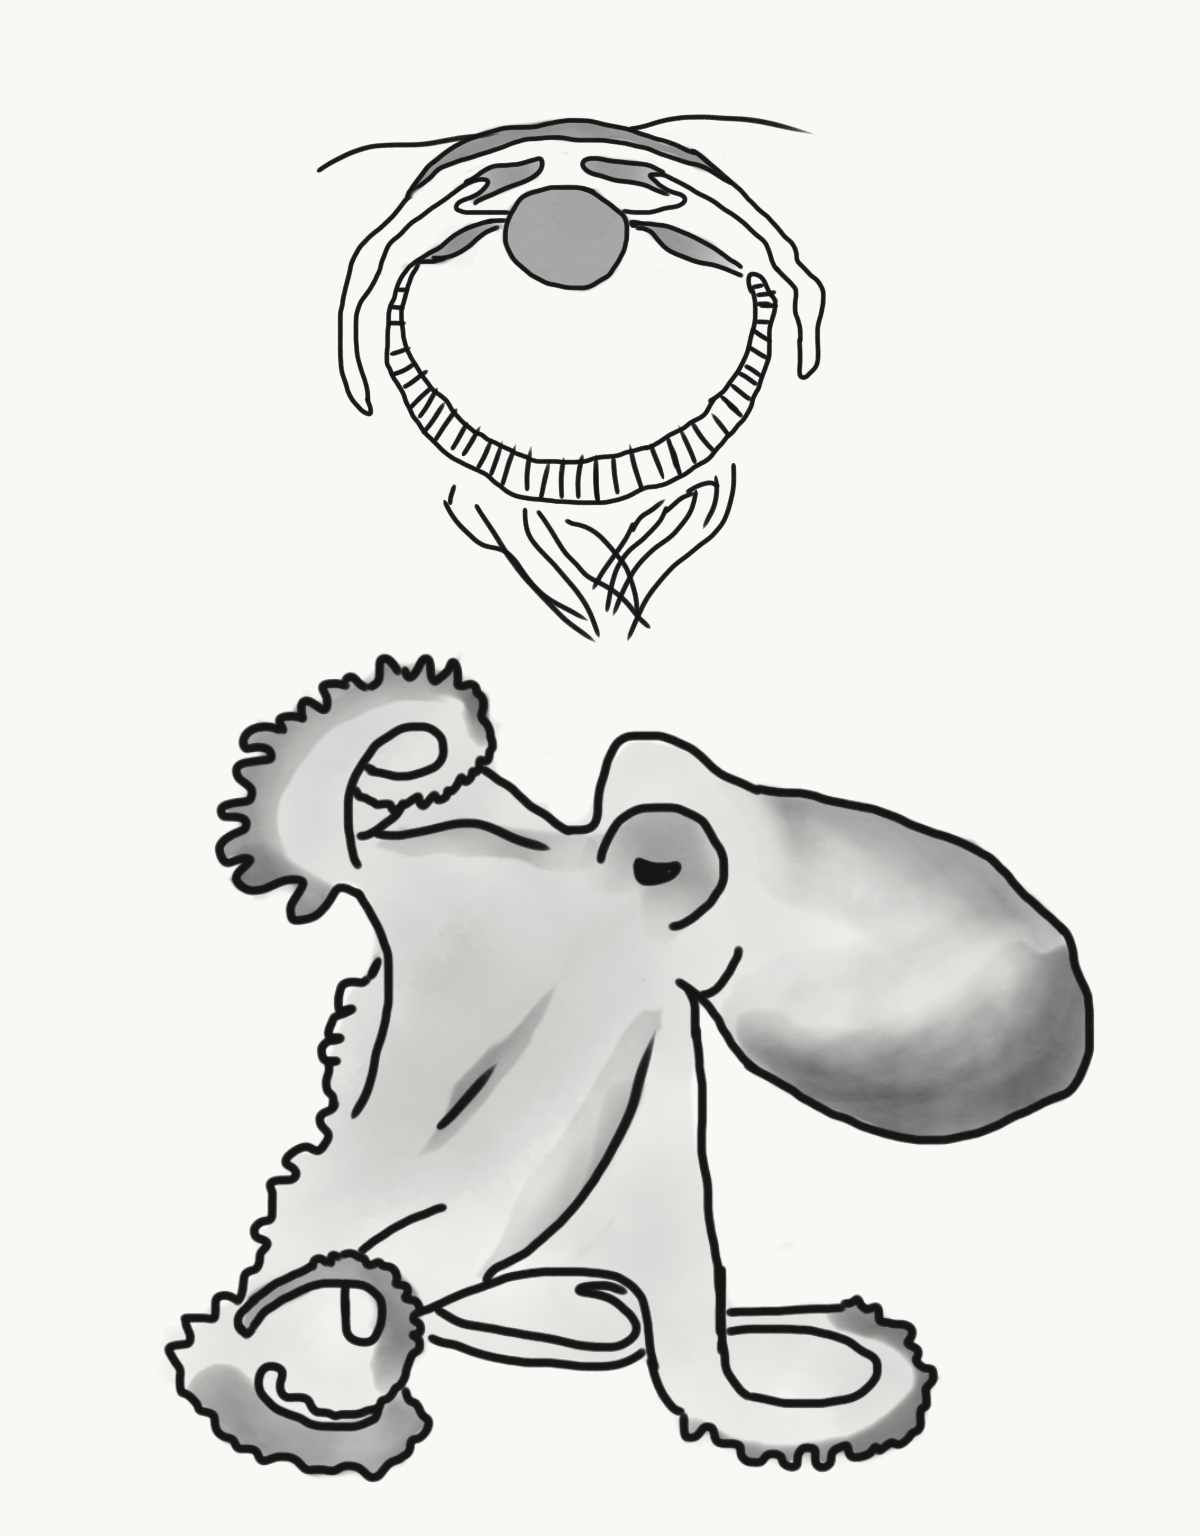
\includegraphics[height=3cm]{img/octopus_eye}%
  }%
}
\setlength{\twosubht}{\ht\twosubbox}

% typeset

\centering

\subcaptionbox{light sensitive  cells in the worm\label{subfig:worm_eye}}{%
  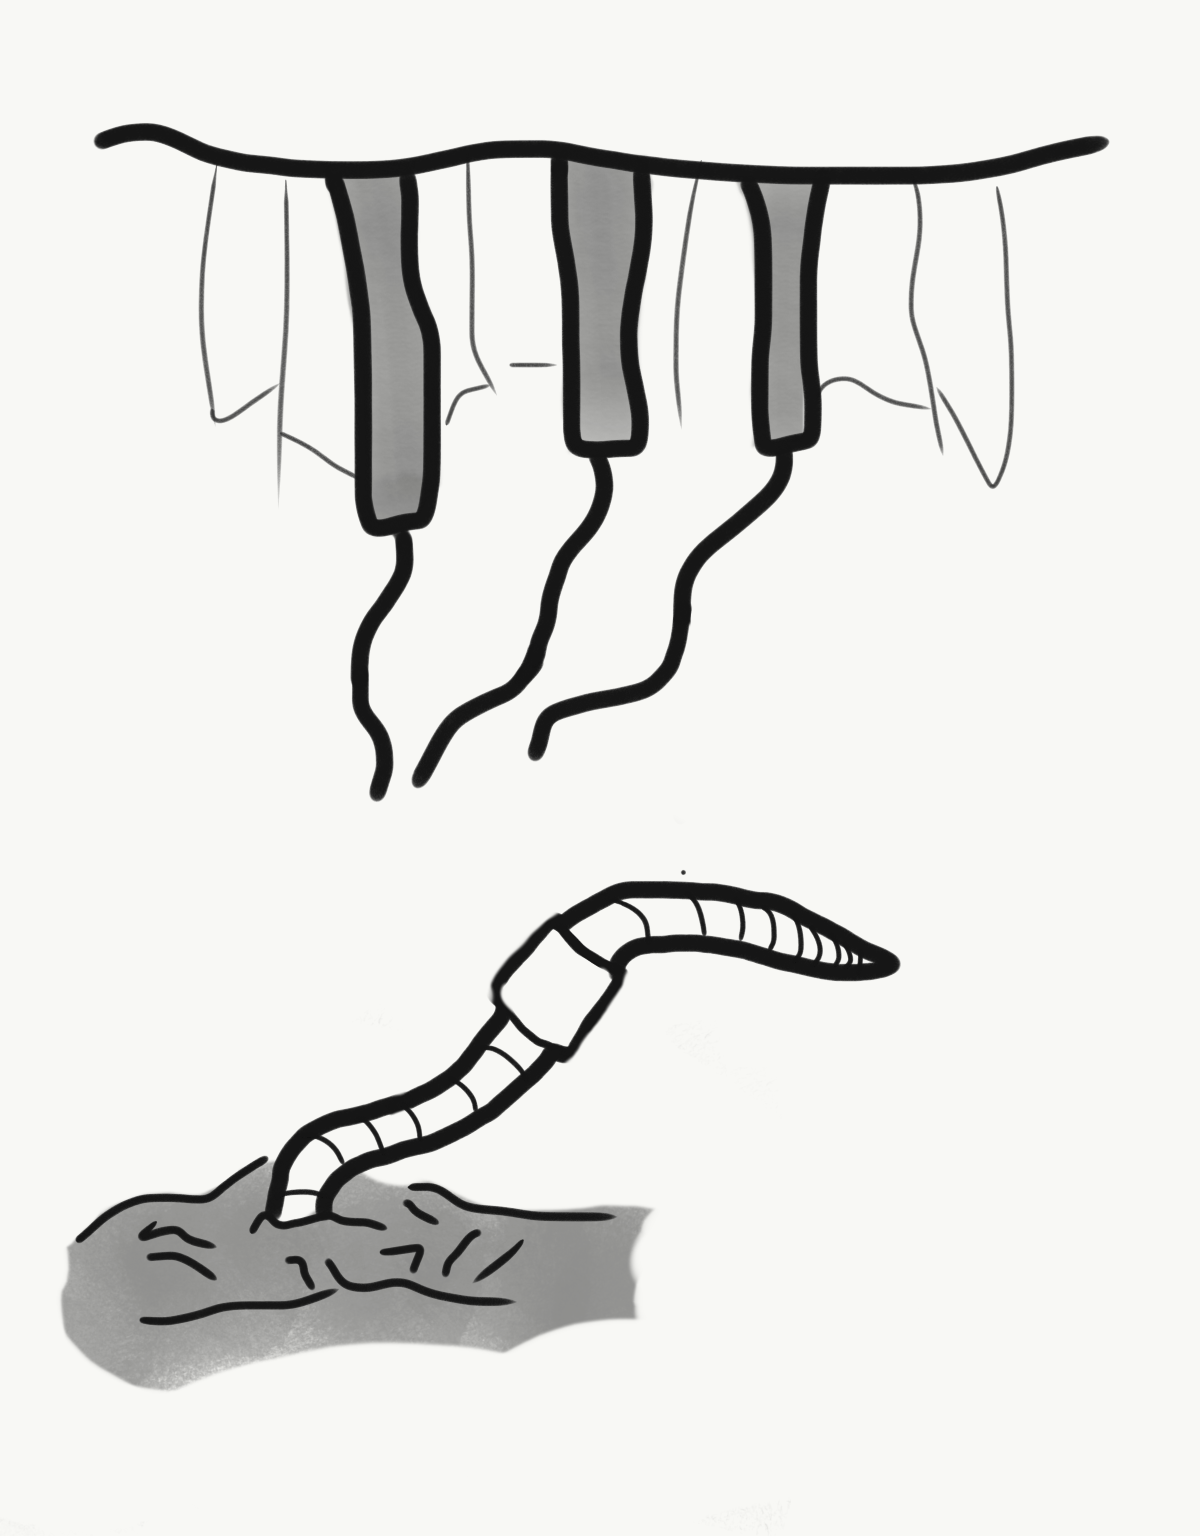
\includegraphics[height=\twosubht]{img/worm_eye}%
}\quad
\subcaptionbox{pit-type eye in the limpet\label{subfig:limpet_eye}}{%
  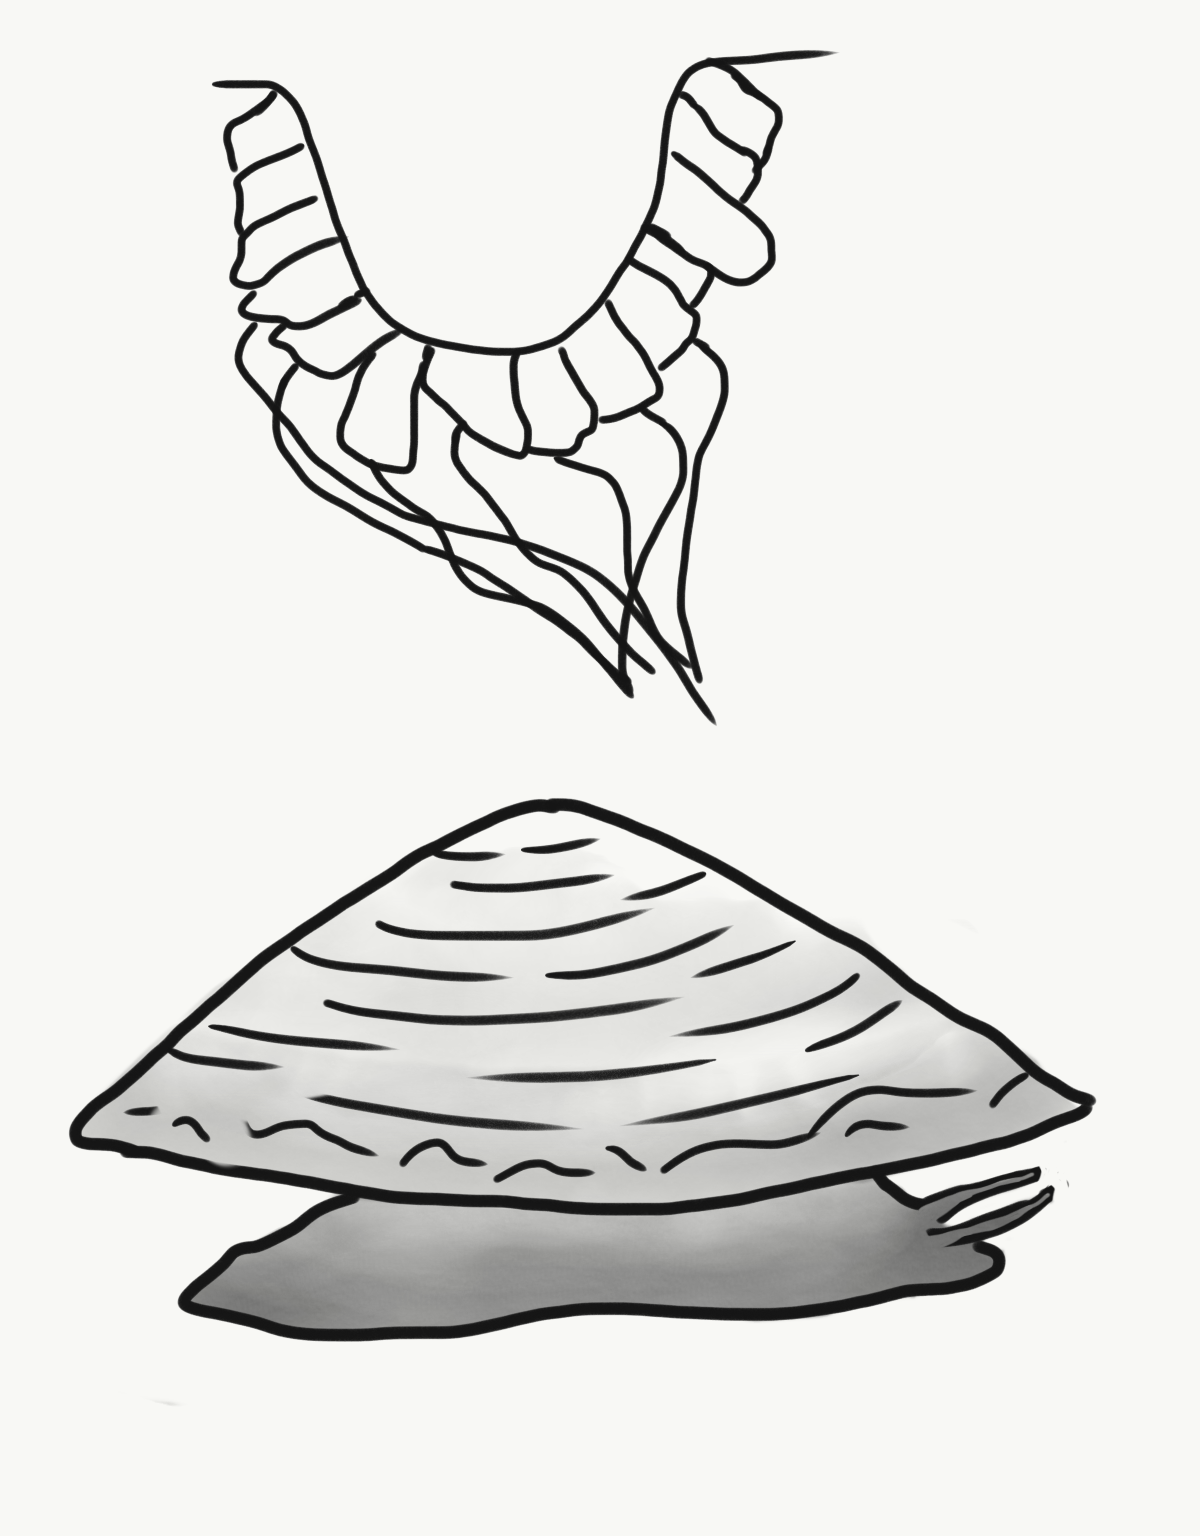
\includegraphics[height=\twosubht]{img/limpet_eye}%
}\quad
\subcaptionbox{pinhole-type eye in the nautilus\label{subfig:nautilus_eye}}{%
  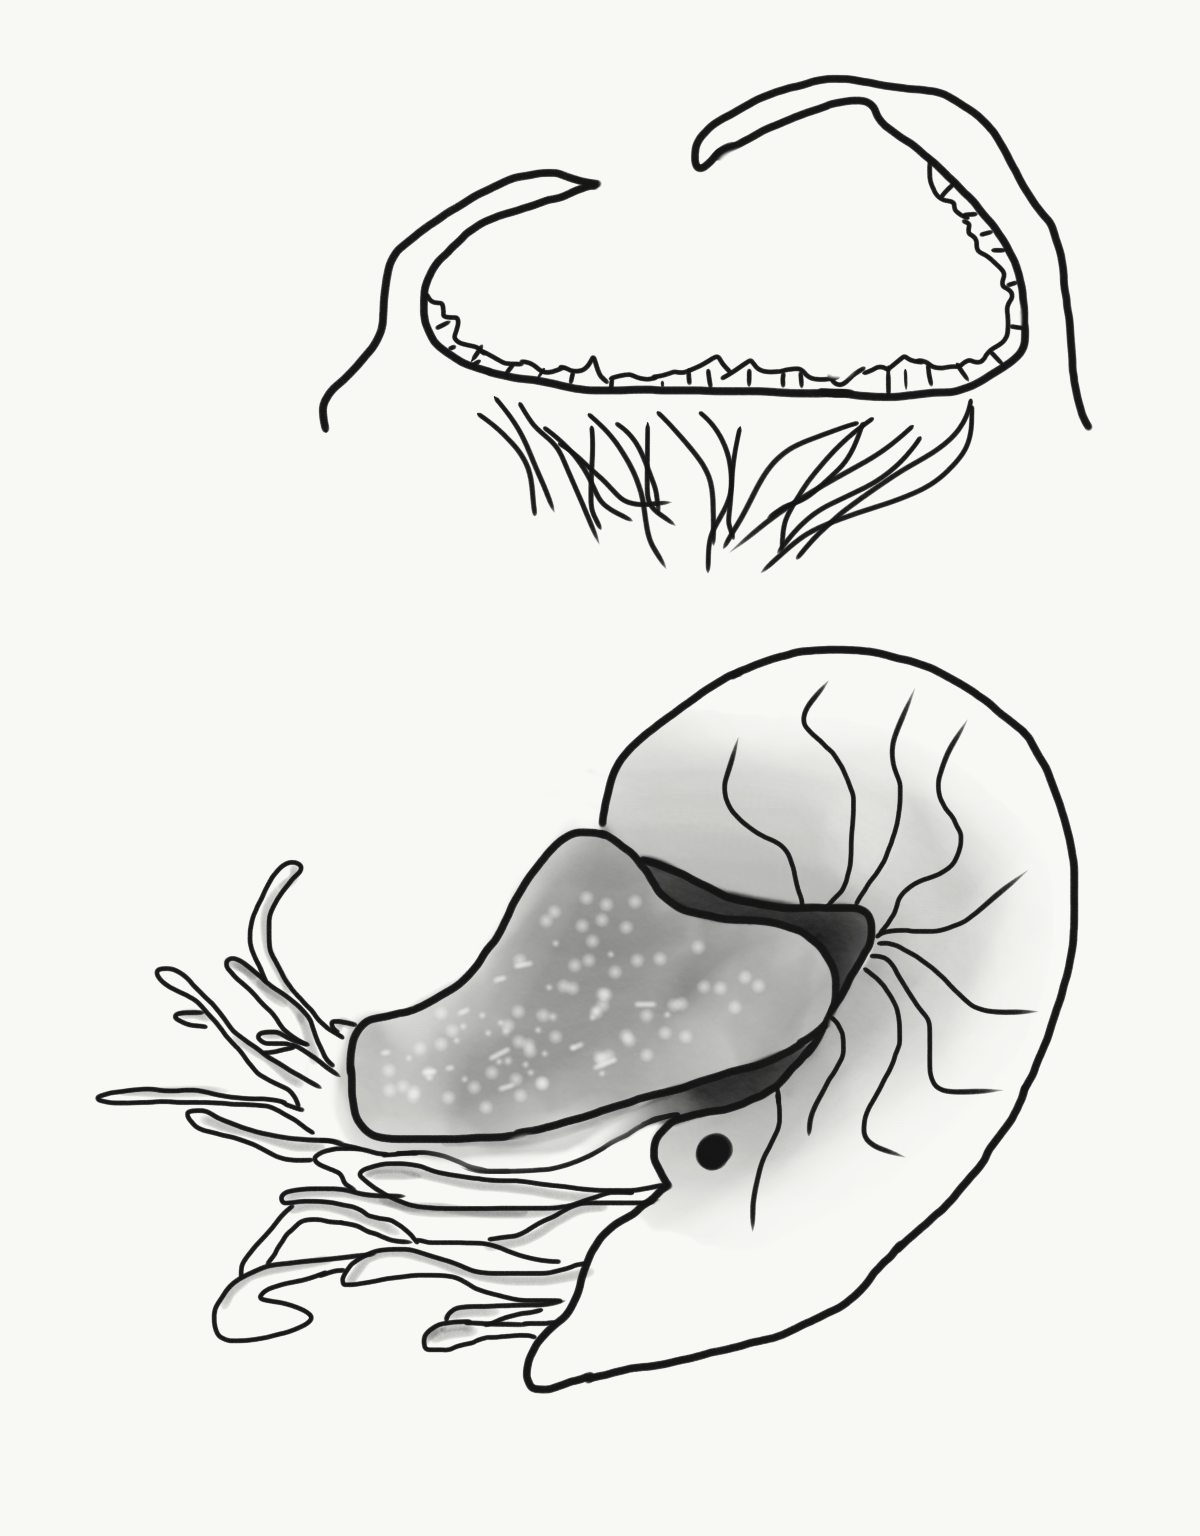
\includegraphics[height=\twosubht]{img/nautilus_eye}%
}\quad
\subcaptionbox{eye with lens in murex \label{subfig:murex_eye}}{%
  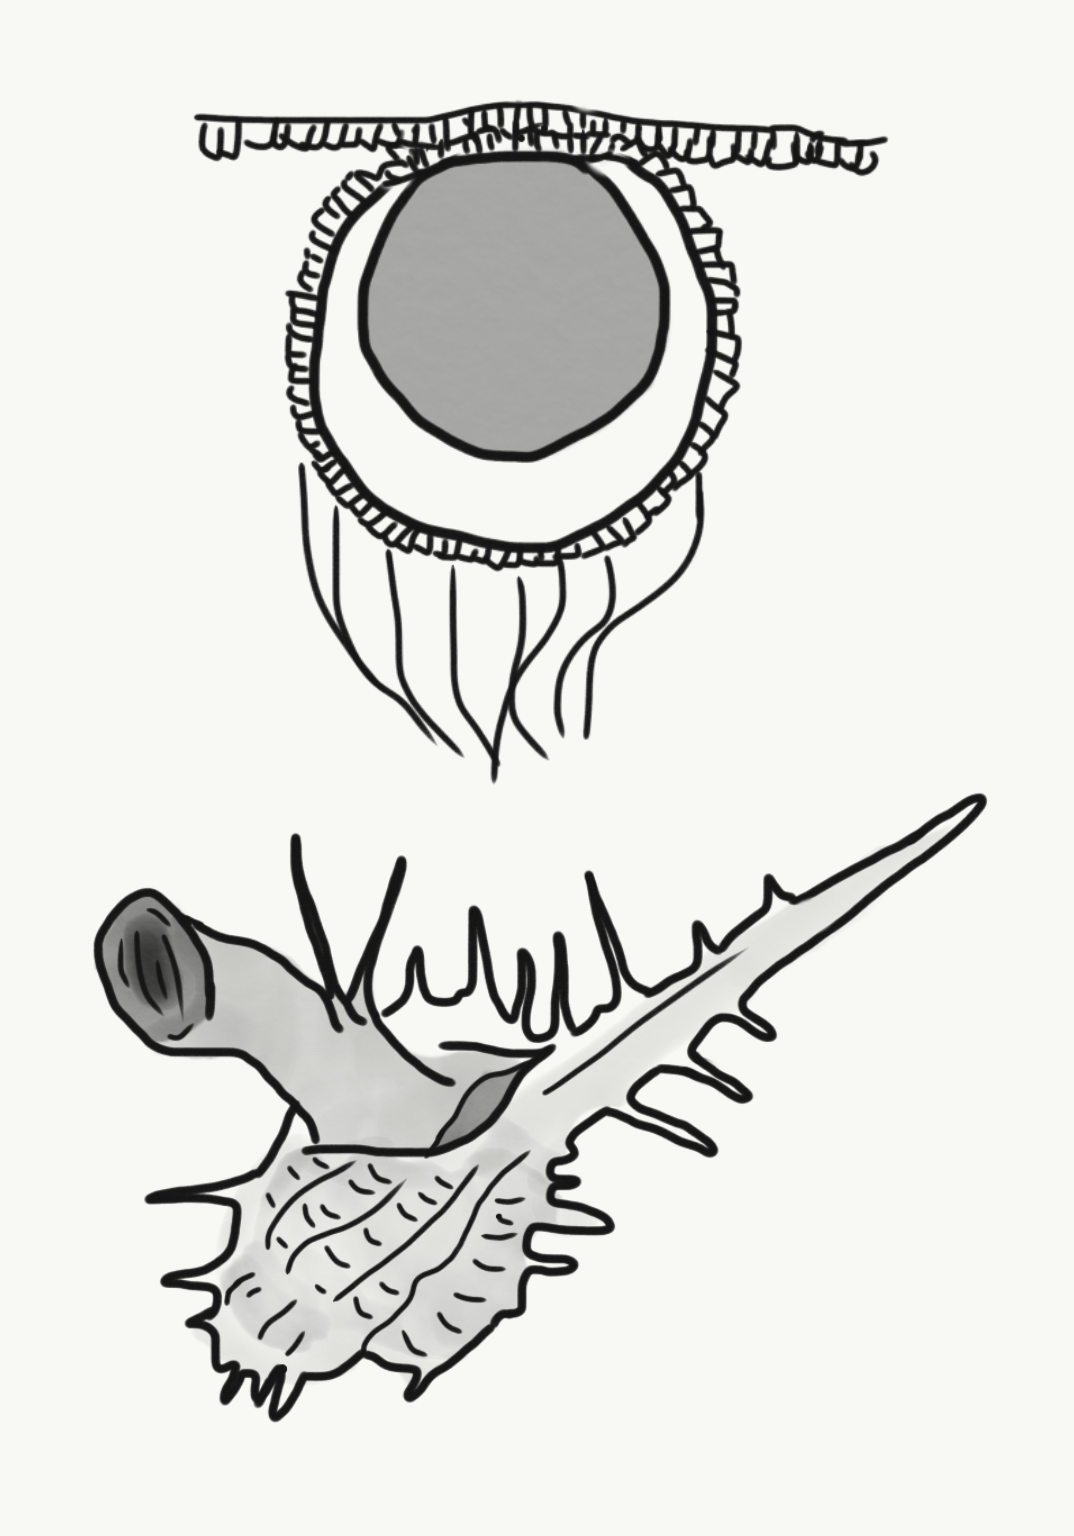
\includegraphics[height=\twosubht]{img/murex_eye}%
}\quad
\subcaptionbox{camera-type eye in the octopus\label{octopus_eye}}{%
  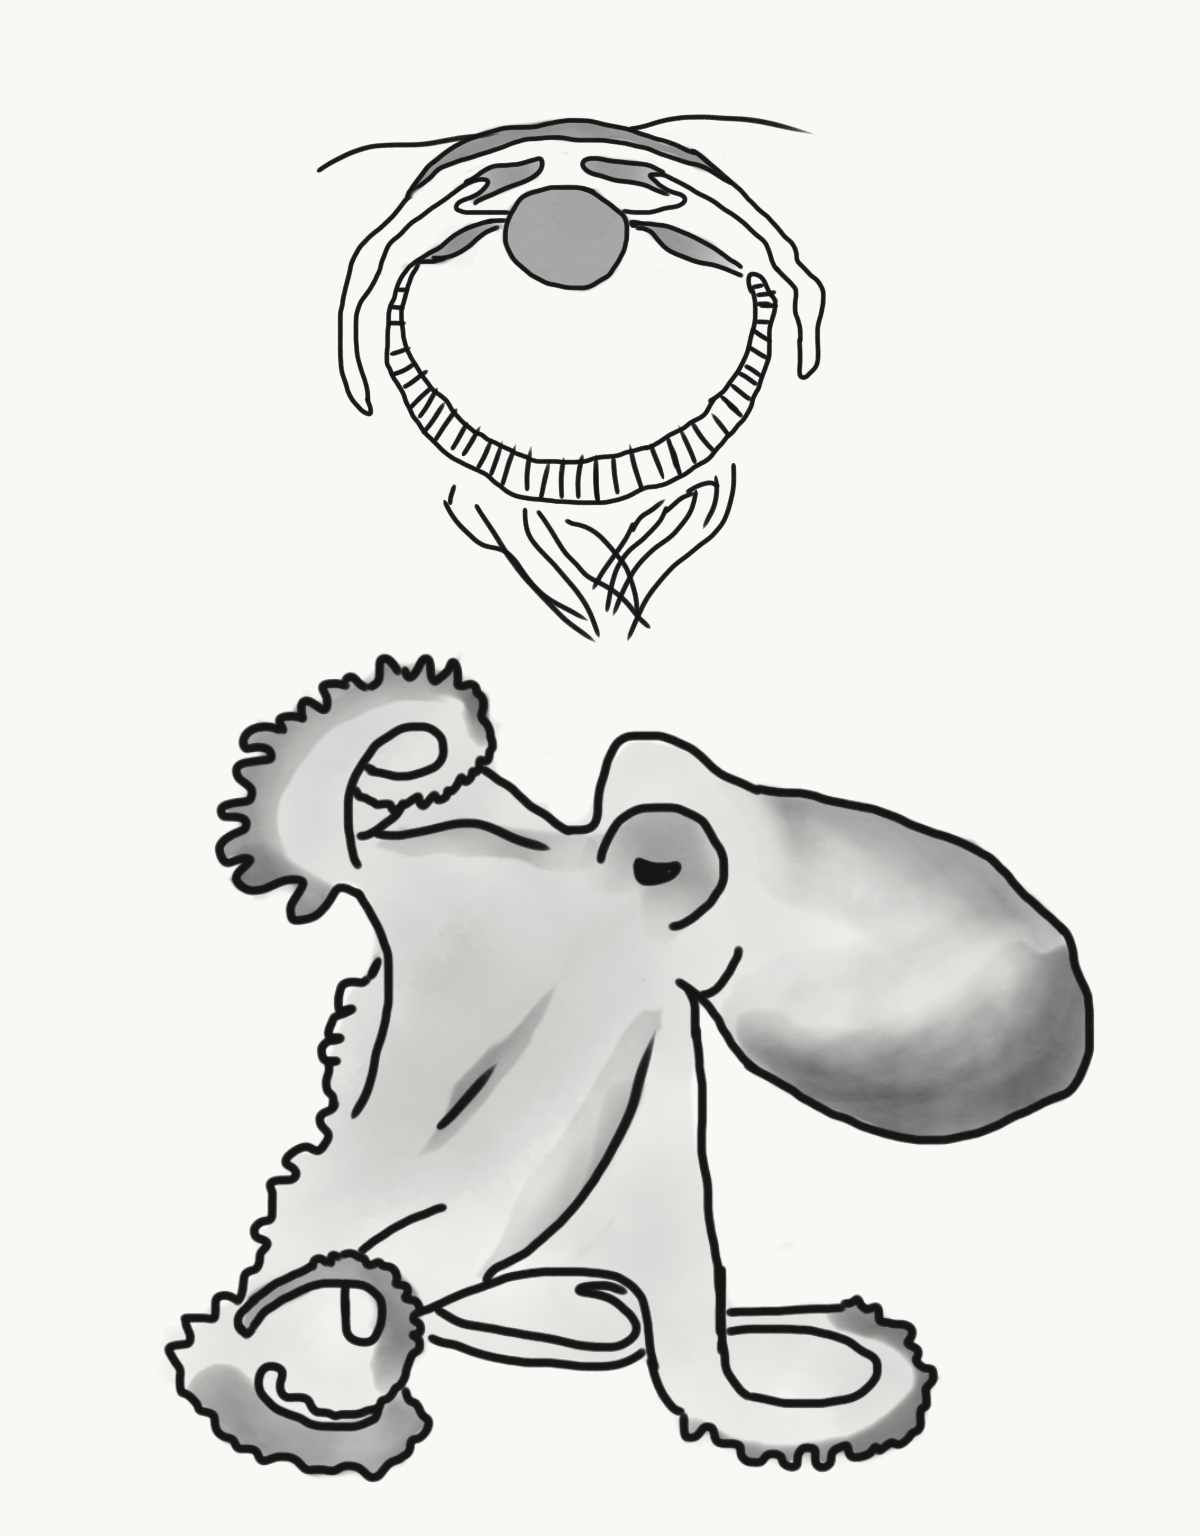
\includegraphics[height=\twosubht]{img/octopus_eye}%
}


\caption{Extant organisms that illustrate several different typese of eyes, which might have provided a potential route of complexification of the ocular organ by evolution \cite{Gregory2008TheOrgans}.}


%    \centering
% 	\begin{minipage}
%         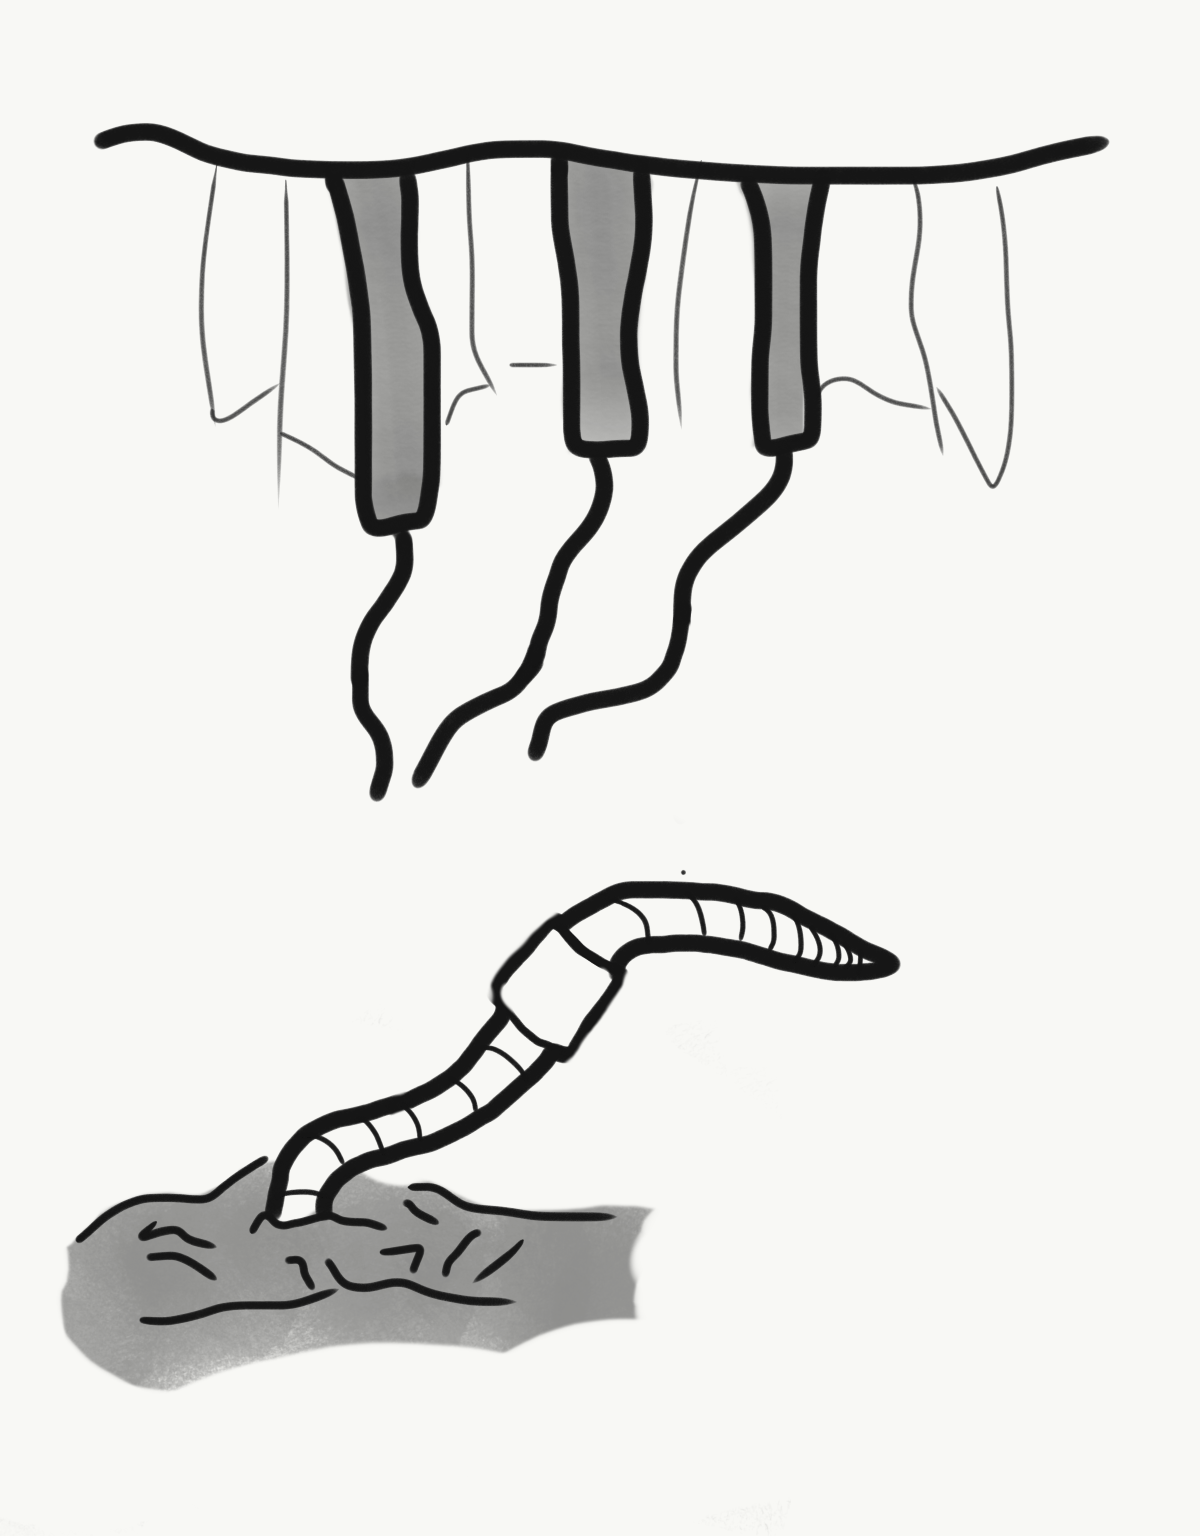
\includegraphics[height=3cm]{img/worm_eye}
%         %\caption{}
%         %\label{subfig:worm_eye}
%     \end{minipage}
%     \begin{minipage}
%         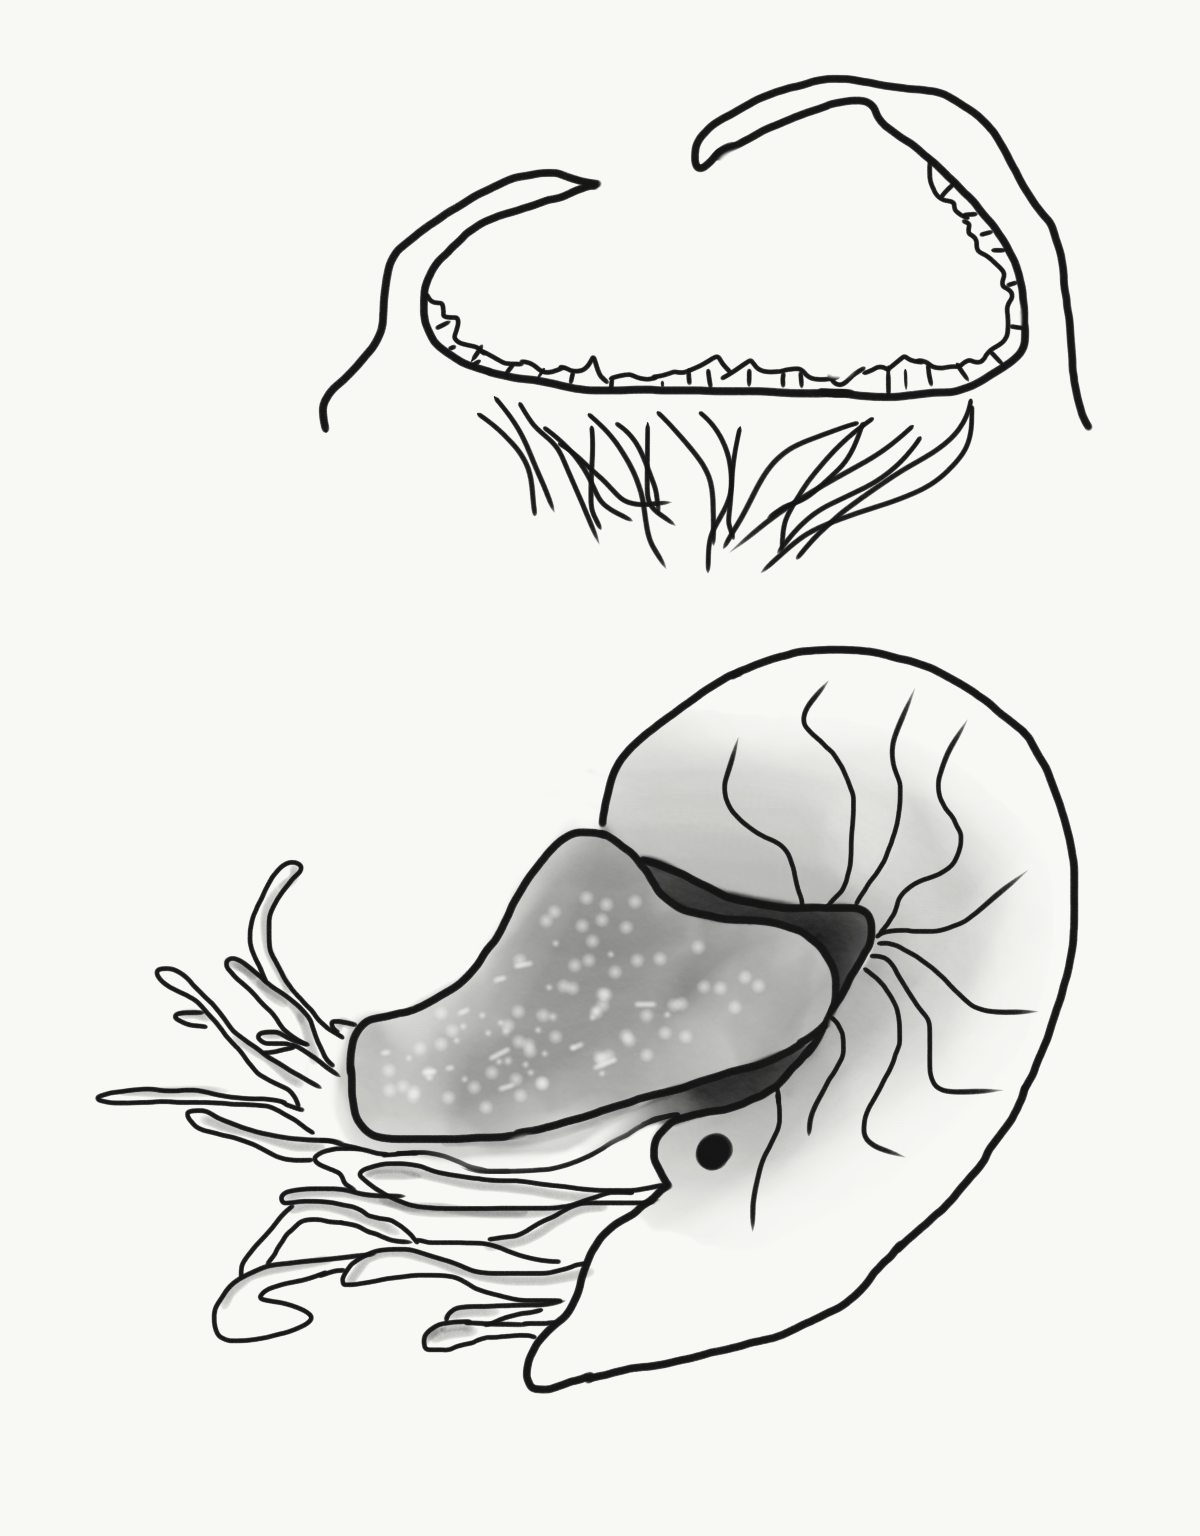
\includegraphics[height=3cm]{img/nautilus_eye}x
%         %\caption{}
%         %\label{subfig:nautilus_eye}
%     \end{minipage}
%     \begin{minipage}
%         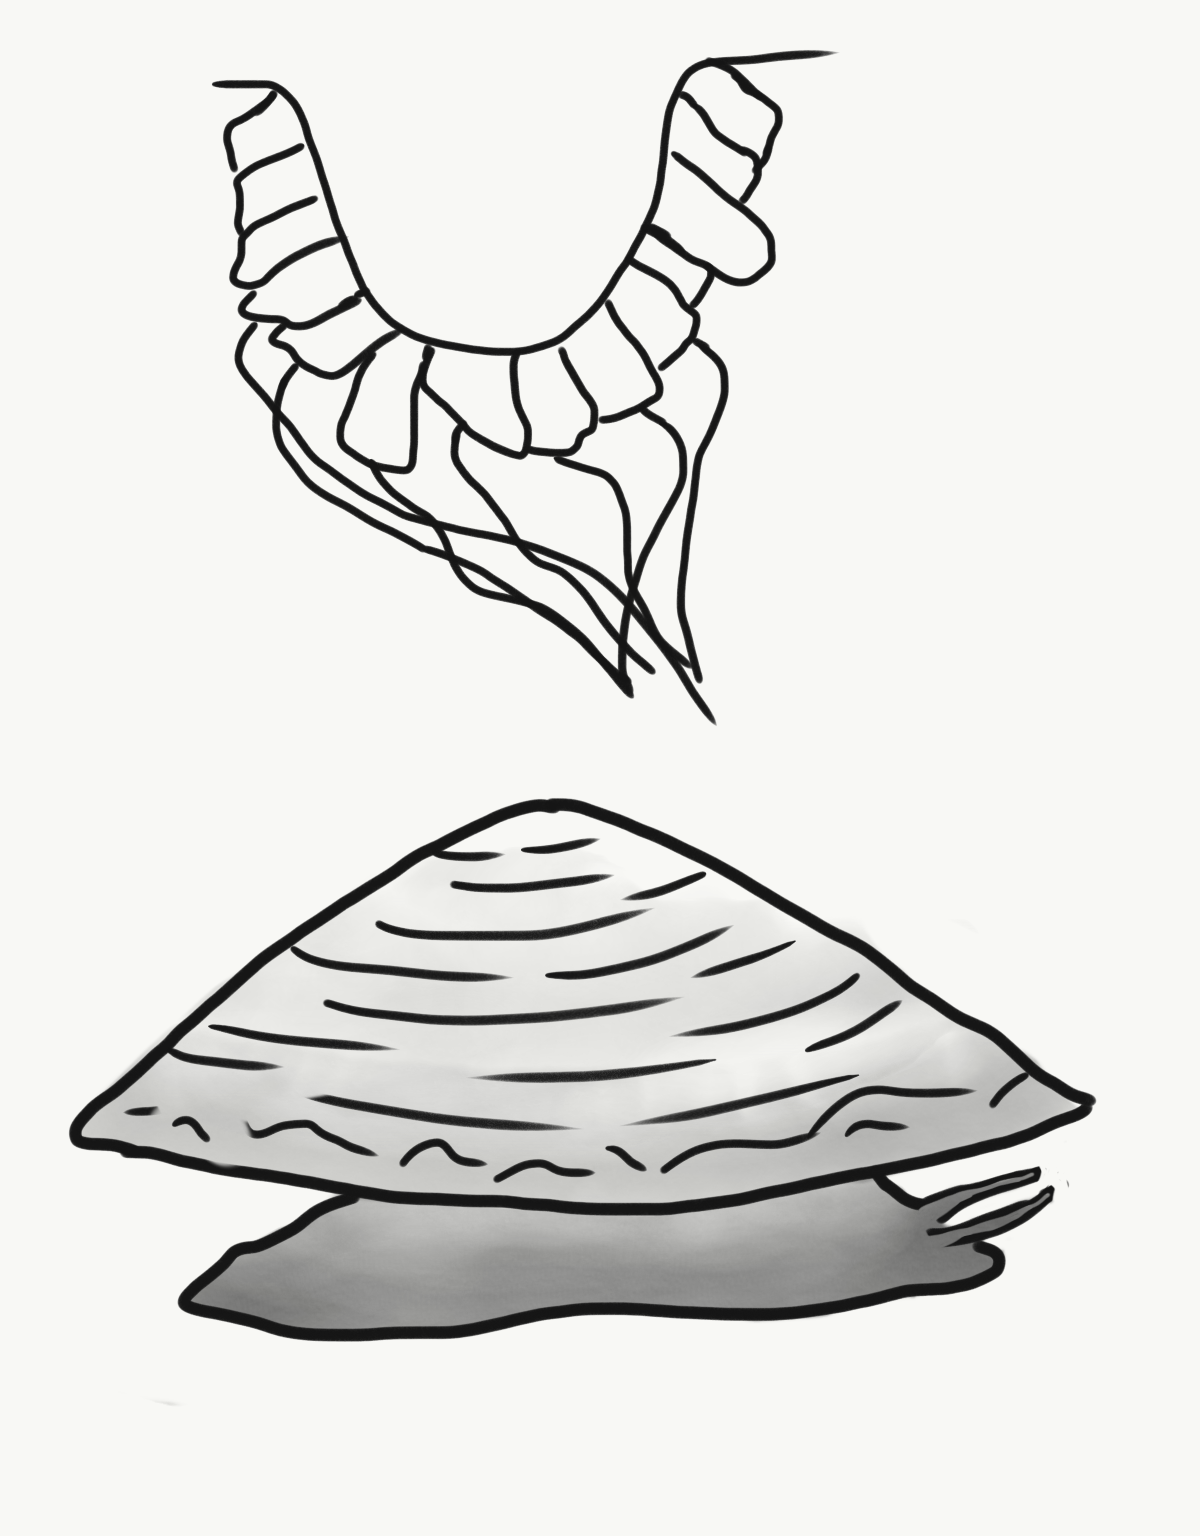
\includegraphics[height=3cm]{img/limpet_eye}
%         %\caption{pit-type eye in the limpet}
%         %\label{subfig:limpet_eye}
%     \end{minipage}
%     \begin{subfigure}
%         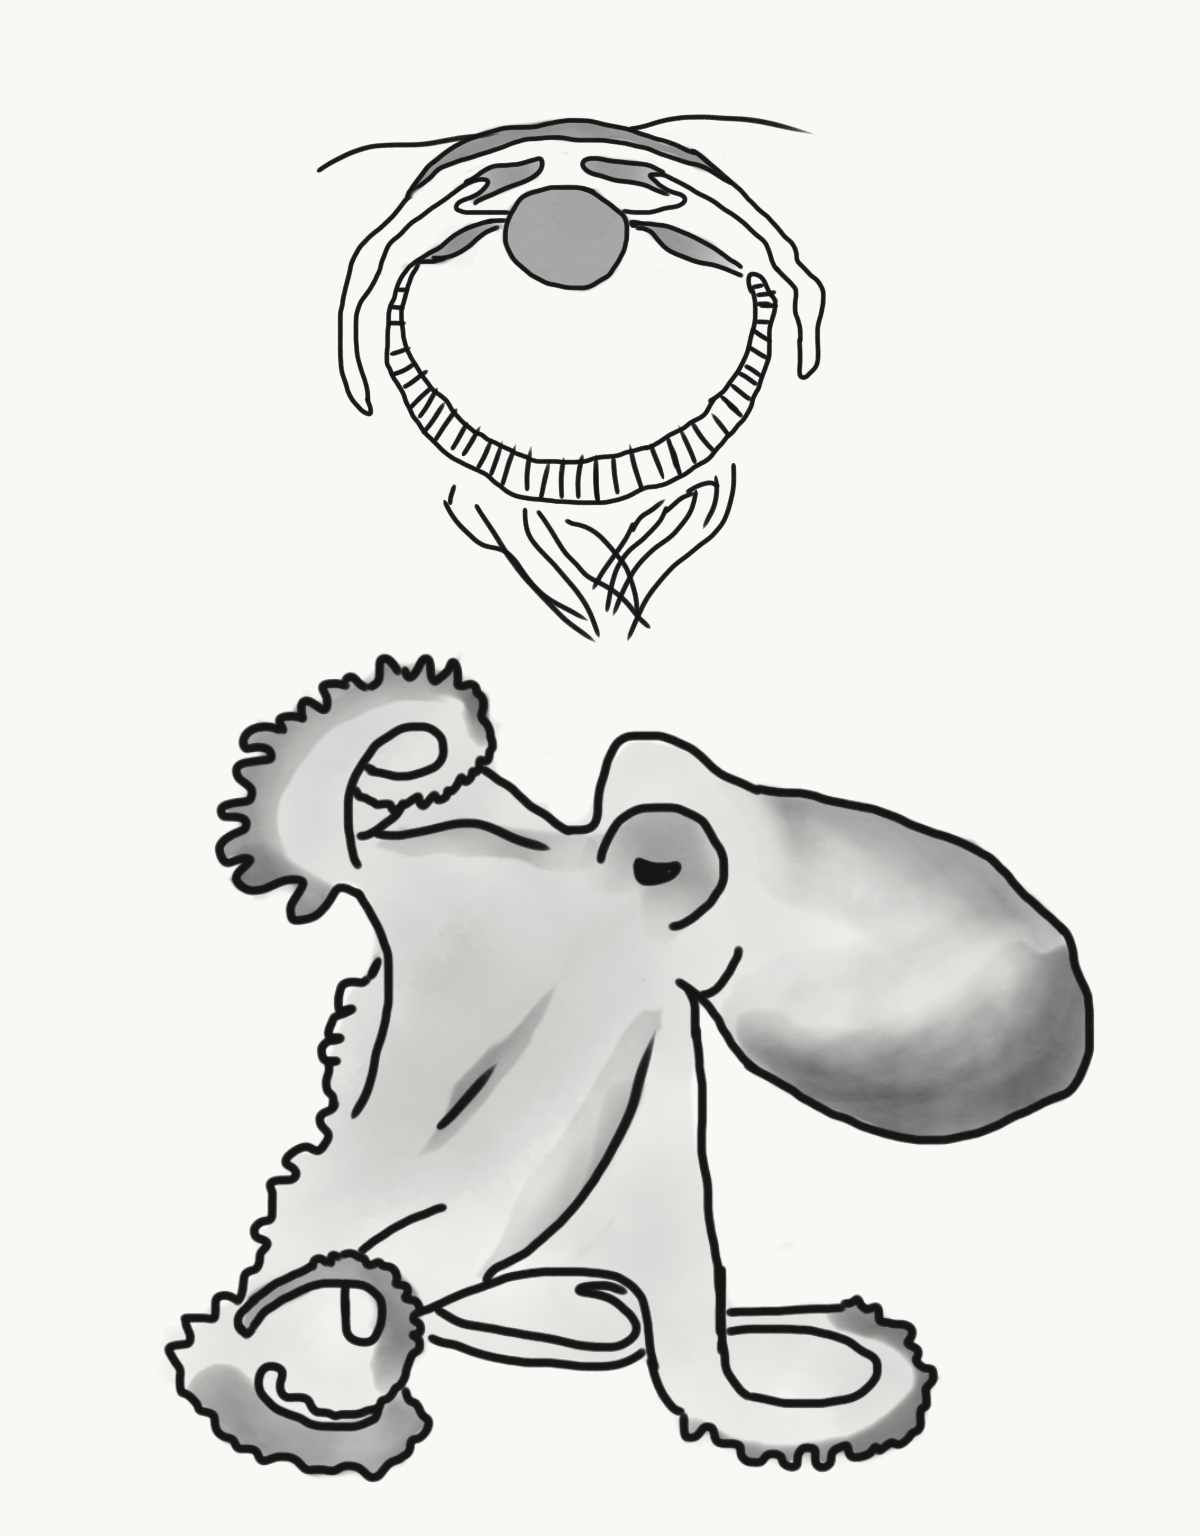
\includegraphics[height=3cm]{img/octopus_eye}
%         %\caption{camera-type eye in the octopus}
%         %\label{subfig:octopus_eye}
%     \end{subfigure}
%   \captionsetup{singlelinecheck=off,justification=raggedright}
%   \caption{Caption words go here.}
  \label{fig:eye_evolution}
\end{figure}